\documentclass[a4paper,8pt,openany]{book}
\usepackage[utf8]{inputenc}
\usepackage[french]{babel}
\usepackage[T1]{fontenc}
\usepackage{graphicx}
\usepackage{titlesec}
\usepackage{amsmath}
\usepackage{amsfonts}

\titleformat{\chapter}[block]
  {\normalfont\Huge\bfseries}% font of number
  {\chaptertitlename\ \thechapter~:}% format of number
  {20pt}% space between number and title
  {\Huge}% font of title

\titlespacing*{\chapter}
  {0pt}%  indent
  {0pt}% space before
  {20pt}% space after
\titlespacing*{\section}
  {0pt}%  indent
  {3.5ex plus 1ex minus .2ex}% space before
  {2.3ex plus .2ex}% space after

\author{Mendy Fatnassi}
\title{Cours de Mathematique en Geometrie}

%%%%%%%%%%%%%%%%%%%%%%%%%%%%%%%%%%%%%%	Page	%%%%%%%%%%%%%%%%%%%%%%%%%%%%%%%%%%%%%%%%
\begin{document}
\maketitle
\tableofcontents

\chapter{Geometrie}
\\
\section{Generalite}
Sur un graphique on a 2 axe l'abscisse en x ,axe horizontale et l'ordonnee en y ,axe verticale .\\
On note une coordonne\'e(x,y).\\


\section{Sin et Cos}



\section{Cercle Trigonometrique}
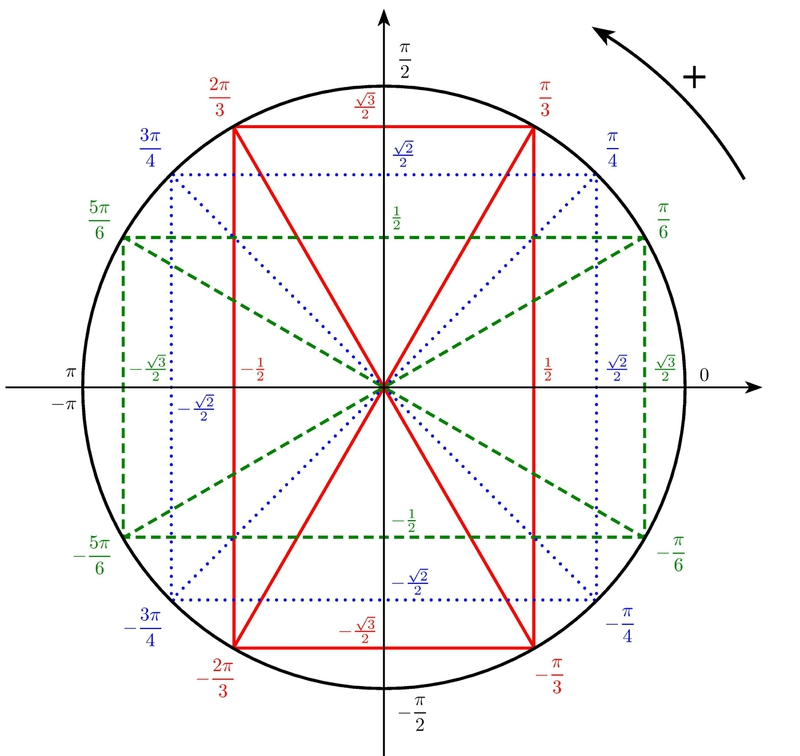
\includegraphics[width=1\textwidth, center]{cercle_trigo.jpg}
\\



\section{vecteur}
\underline{Vocabulaire}\\
Colineaire : Si on a 3 vecteurs non nul sont colineaire cela veux dire que les 3points sont alignes .\\
Orthogonal : ON dit que 2 droit sont perpendiculaire quand elle forme un angle droit sur un meme plans mais si ces 2 droites sont sur un plans de dimenions 3 , les 2 droites sont perpendiculaire mais ne se touche pas on dit qu'elle sont orthogonal.\\
coplanaire : les droites sont situé dans un meme plans .\\

Le vecteur \vec{u} de coordonnees (2,-3,1) est le vecteur donne par la somme 2\vec{i}-3\vec{j}+\vec{k} .\\
La norme de \vec{u} est donnee par \lVert u \rVert = \sqrt{2^2+(-3)^2+1^2}=\sqrt{14}\\
\\

\subsection{Produit Scalaire} :\\
On considere les vecteurs \overrightarrow{AB} et \overrightarrow{AC} .Soient 3point A,B,C .Le produit scalaire de ces deux vecteurs note \overrightarrow{AB}.\overrightarrow{AC} est le scalaire reel : \lVert \overrightarrow{AB} \rVert.\lVert \overrightarrow{AC} \rVert.\cos(BAC) .\\
\\
\underline{Avec les coordonnes composante}:\\
Lorsque les vecteurs ont leurs coordonnees dans une base orthonorme le calcule du produit scalaire est direct .
Soient \vec{u}(u1,u2,u3) et \vec{v}(v_1,v_2,v_3) on a \vec{u}.\vec{v}=u_1v_1+u_2v_2+u_3v_3 .\\
\\
2 vecteurs \overrightarrow{AB} et \overrightarrow{AC} sont orthogonaux ssi \overrightarrow{Ab}.\overrightarrow{AC}=0 .\\
Si 2 vecteurs \overrightarrow{AB} et \overrightarrow{AC} sont colineaire et de meme sens \overrightarrow{AB}.\overrightarrow{AC}=\lVert \overrightarrow{AB} \rVert.\lVert \overrightarrow{AC} \rVert.cos(0)=\lVert \overrightarrow{AB} \rVert.\lVert \overrightarrow{AC} \rVert \\

\subsection{Produit vectoriel}
Le produit vectoriel de 2 vect a 3 coordonees (dimensions) \vec{u} et \vec{v} est l'unique vecteur \vec{w} tel que :\\
-\vec{w} est orthogonal aux 2 vecteur \vec{u} et \vec{v}.\\
-La base (\vec{u},\vec{v},\vec{w}) est de sens direct (regle 3 doigt x,y,z).\\
-\lVert \vec{w} \rVert = \lVert \vec{u} \rVert.\lVert \vec{v} \rVert.|\sin(\vec{u},\vec{v})| \\
\\
Il se note ainsi : \lVert \vec{u} \wedge \vec{v} \rVert = \lVert \vec{u} \rVert.\lVert \vec{v} \rVert.sin(\frac{\pi}{2}) \\
\\
\underline{avec les coordonnees}:\\
pour calculer le produit vectoriel avec \vec{u}=(u1,u2,u3) et \vec{v}=(v1,v2,v3).\\
\lVert \vec{u} \wedge \vec{v} \rVert = (u2.v2-u3.v2 ; u3.v1-u1.v3 ; u1.v2-u2.v1) on fait des produit en croix.\\



\subsection{Barycentre}: Soient A_1,...,A_n des points de l'espace et a_1,...,a_n des scalires de somme non nulle.\\
Le barycentre des point A_1,...,A_n affecte des coefficients  a_1,...,a_n est l'unique point G tel que $\sum_{i=1}^{n}(a_i\vec{GA_i})=\vec{0}$ , quand tous les coef. sont a 1 on parle d'isobarrycentre.\\
exemple : en 2 dim. , soient les points A(-2;-1),B(0;3)et C(4;1) cherchons G=bar((A,1),(B,3),(C,2))=1+3-2=2 \neq 0 donc G existe.On a la relation  \lVert \vec{GA} \rVert+3 \lVert \vec{GB} \rVert-2 \lVert \vec{GC} \rVert=\vec{0} .\\
En etudiant les coordonnées , on a : \\
(xa-xg)+3(xb-xg)-2(xc-xg)=0 \Leftrightarrow (-2-xg-3xg-8-2xg)=0 \Leftrightarrow (2xg=-10) \Leftrightarrow (xg=-5)\\
(ya-yg)+3(yb-yg)-2(yc-yg)=0 \Leftrightarrow (-1-yg+9-3yg-2+2yg)=0 \Leftrightarrow (2yg=6) \Leftrightarrow (yg=3)\\
\\


\end{document}